\section{Conclusioni}
In conclusione, il prototipo sviluppato rappresenta un passo significativo verso la fondazione di una start-up innovativa. La sua realizzazione ha offerto un'opportunità preziosa per comprendere a fondo l'idea e presentarla a potenziali investitori, nonché per acquisire abilità tecniche e di business nell'ambito dell'Internet of Things (IoT) e dell'ecosistema Amazon AWS. Quest'ultimo è fondamentale per il successo del progetto, grazie alla sua flessibilità d'utilizzo e all'ampia gamma di servizi di supporto.
%
Durante lo sviluppo del prototipo, sono emerse alcune sfide cruciali che richiederanno ulteriori perfezionamenti per migliorare il prodotto. In particolare, il linguaggio di programmazione Java utilizzato per la componente di sensibilizzazione si è dimostrato poco efficiente, per cui sarà opportuno riscrivere il software della unità di controllo in un linguaggio più performante, come C. Inoltre, sarà importante individuare una soluzione sul mercato che sia meno costosa del raspberry utilizzato, ad esempio un microcontrollore.
%
Nonostante i commenti positivi ricevuti dalle diverse comunità di utenti, i sensori acquistati hanno mostrato un rapporto qualità-prezzo insoddisfacente, per cui sarà necessario effettuare una valutazione più approfondita dei dispositivi IoT per individuare alternative più economiche ma comunque affidabili.
%
Per quanto riguarda il futuro del progetto, sarà imprescindibile sviluppare un prodotto più performante e conveniente, così da soddisfare le esigenze dei clienti. Questo dovrà inoltre essere in grado di scalare in modo efficiente in risposta a un aumento improvviso delle richieste di sottoscrizione, al fine di gestire adeguatamente la grande quantità di dati generati dalle centraline.
%
Infine, sarà importante chiarificare le opportunità di crescita e espansione dell'IoT nel settore alberghiero, per posizionarsi in modo vantaggioso e conquistare una quota significativa del mercato.

\begin{figure}[H]
    \begin{minipage}{0.37\textwidth}
    \hspace*{-0.3cm}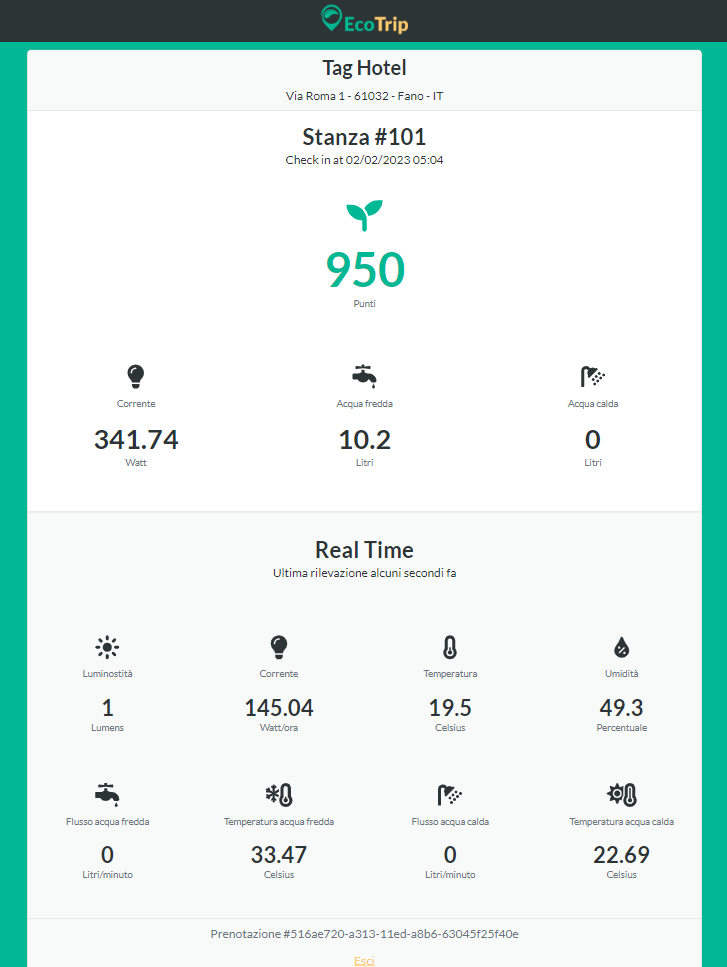
\includegraphics[width=\textwidth]{app-screen.png}
    \caption[contextmap]{Screenshot dell'app}
    \label{fig:app1}
    \end{minipage}
    \begin{minipage}{0.62\textwidth}
    \hspace*{0.5cm}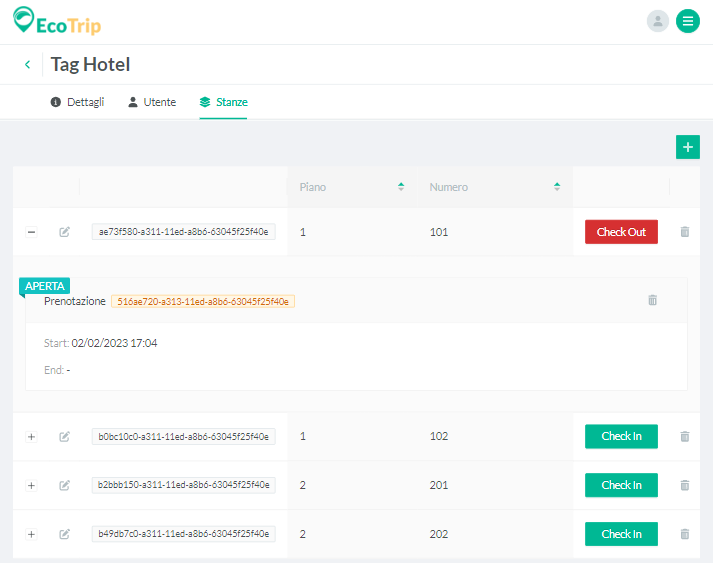
\includegraphics[width=\textwidth]{cp-screen.png}
    \caption[contextmap]{Screenshot del pannello}
    \label{fig:app2}
    \end{minipage}
    \centering
\end{figure}

\begin{figure}[H]
    \begin{minipage}{0.40\textwidth}
    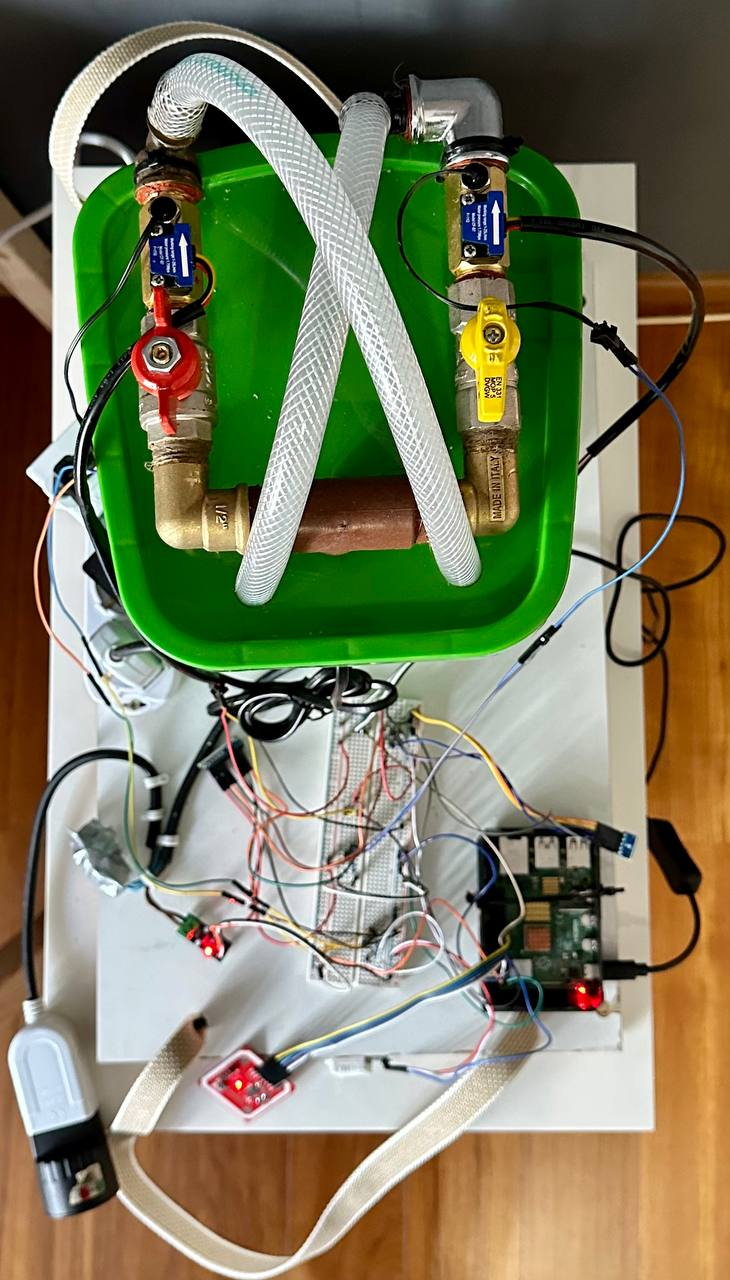
\includegraphics[width=\textwidth]{foto1.jpg}
    \label{fig:foto1}
    \end{minipage}
    \begin{minipage}{0.57\textwidth}
    \hspace*{0.5cm}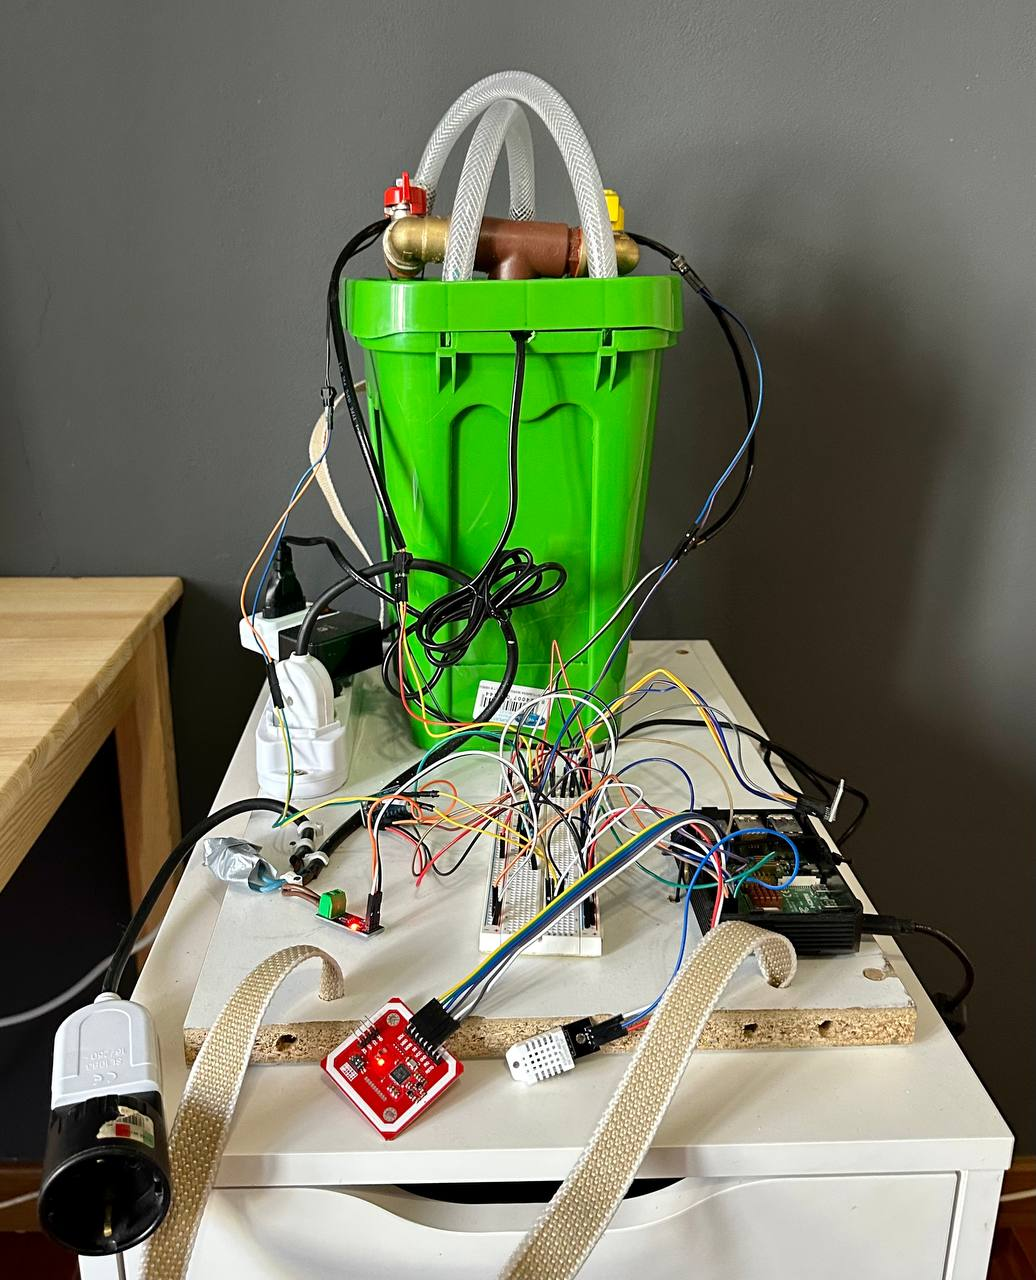
\includegraphics[width=\textwidth]{foto2.jpg}
    \label{fig:foto2}
    \end{minipage}
    \centering
    \caption[contextmap]{Foto del prototipo realizzato}
\end{figure}